\documentclass[tikz,border=10pt]{standalone}
\usepackage{amsmath,amssymb}
\usepackage{tikz}
\usetikzlibrary{arrows.meta,calc,decorations.pathreplacing,decorations.pathmorphing,patterns,shapes.geometric,positioning,shadings}

\begin{document}
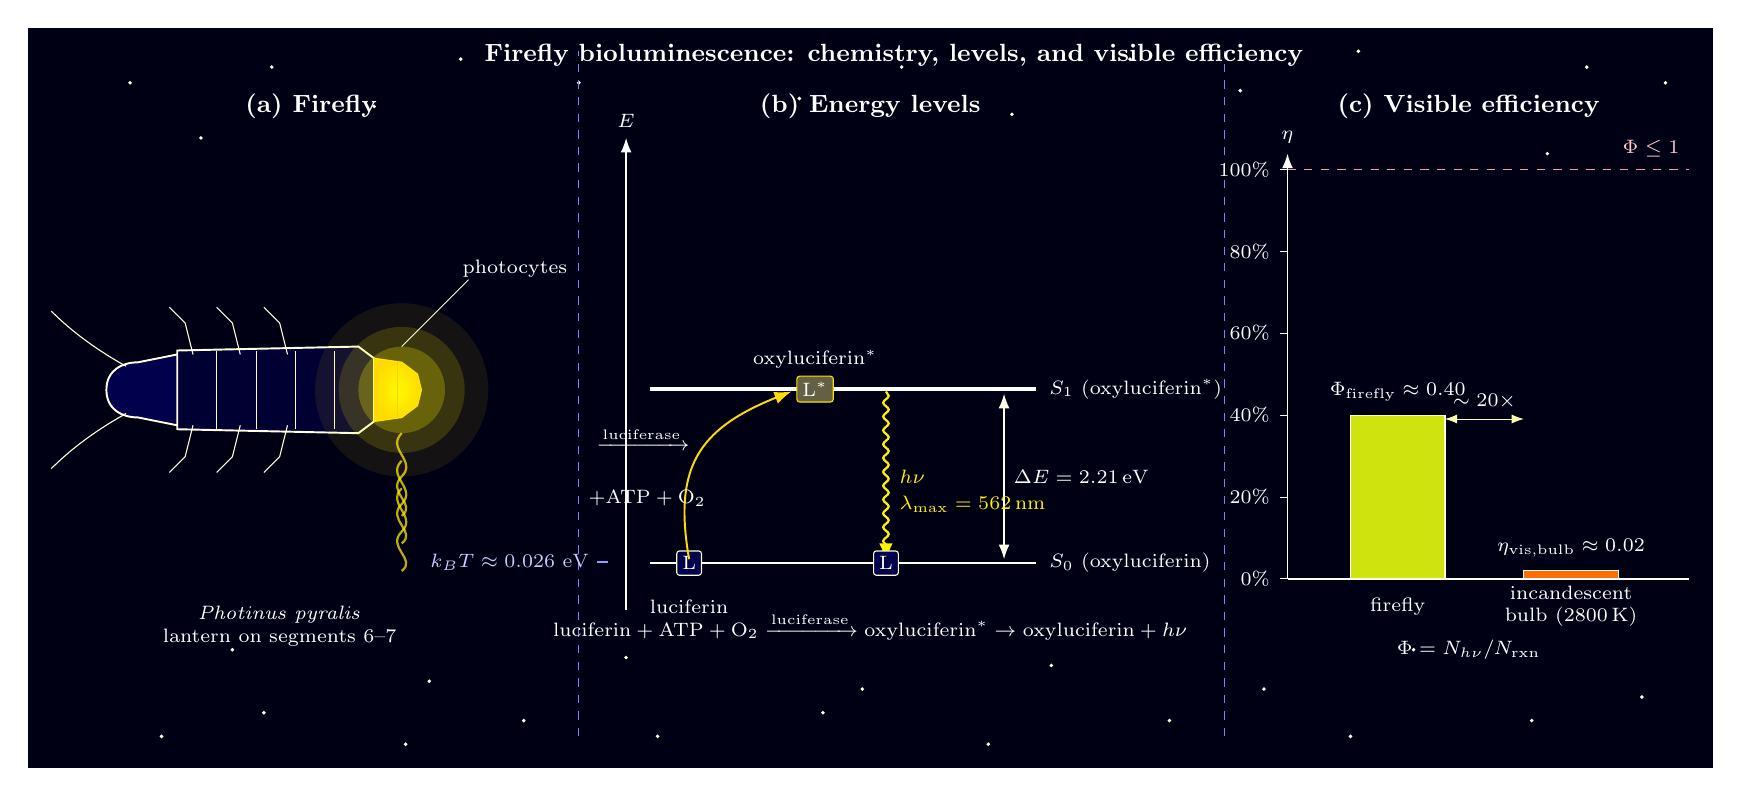
\begin{tikzpicture}[
  >=Latex,
  font=\footnotesize
]

% ============================================================
% Dark night-sky background
% ============================================================
\fill[black!92!blue] (-1,-4.8) rectangle (20.4,4.6);

% stars
\foreach \x/\y in {0.3/3.9, 1.2/3.2, 2.1/4.1, 3.4/3.6, 4.5/4.2,
                   6.0/3.9, 7.3/4.3, 8.8/3.7, 10.1/4.1, 11.5/3.5,
                   13.0/4.2, 14.4/3.8, 15.9/4.3, 17.2/3.6, 18.8/4.1,
                   0.7/-4.4, 2.0/-4.1, 3.8/-4.5, 5.3/-4.2, 7.0/-4.4,
                   9.1/-4.1, 11.2/-4.5, 13.5/-4.2, 15.8/-4.4, 18.1/-4.2,
                   19.5/-3.9, 19.8/3.9, 18.3/3.0, 16.6/-3.3, 14.7/-3.8,
                   12.0/-3.5, 9.6/-3.8, 6.6/-3.4, 4.1/-3.7, 1.6/-3.3}
  {\fill[white!90!yellow] (\x,\y) circle (0.025);}

% ============================================================
% LEFT PANEL: Firefly
% ============================================================
\begin{scope}[shift={(0,0)}]

  \node[white,font=\small\bfseries] at (2.6,3.6) {(a) Firefly};

  % body - elongated ellipse (length:width roughly 3:1)
  % total length ~ 4, width ~ 1.3
  % head at left, lantern at right-end (last 1/4)
  \coordinate (HeadL) at (0.4,0);
  \coordinate (TailR) at (4.4,0);

  % thorax/head region
  \draw[line width=0.7pt, white!90!yellow, fill=black!70!blue]
    (0.4,0.35) .. controls (0.2,0.35) and (0.0,0.25) .. (0.0,0)
    .. controls (0.0,-0.25) and (0.2,-0.35) .. (0.4,-0.35)
    -- (0.9,-0.45)
    .. controls (1.1,-0.5) and (1.1,0.5) .. (0.9,0.45) -- cycle;

  % antennae
  \draw[line width=0.4pt, white!85!yellow] (0.25,0.3) .. controls (-0.2,0.55) and (-0.5,0.8) .. (-0.7,1.0);
  \draw[line width=0.4pt, white!85!yellow] (0.25,-0.3) .. controls (-0.2,-0.55) and (-0.5,-0.8) .. (-0.7,-1.0);

  % abdomen (segments 2-7)
  \draw[line width=0.7pt, white!90!yellow, fill=black!80!blue]
    (0.9,0.5) -- (3.2,0.55) -- (3.4,0.4) -- (3.4,-0.4) -- (3.2,-0.55) -- (0.9,-0.5) -- cycle;

  % segment lines
  \foreach \x in {1.4,1.9,2.4,2.9}
    \draw[line width=0.3pt, white!75!yellow] (\x,-0.5) -- (\x,0.5);

  % last two segments (lantern) - segments 6,7 - yellow glowing
  \shade[inner color=yellow, outer color=yellow!60!orange]
    (3.4,-0.4) -- (3.4,0.4) -- (3.75,0.35) -- (3.95,0.2) -- (4.0,0) -- (3.95,-0.2) -- (3.75,-0.35) -- cycle;

  % outline of lantern
  \draw[line width=0.5pt, yellow!80!orange]
    (3.4,0.4) -- (3.75,0.35) -- (3.95,0.2) -- (4.0,0) -- (3.95,-0.2) -- (3.75,-0.35) -- (3.4,-0.4);

  % segment line in lantern
  \draw[line width=0.3pt, yellow!50!orange] (3.7,-0.37) -- (3.7,0.37);

  % glow halo
  \foreach \r/\o in {0.55/25,0.8/15,1.1/8}
    \fill[yellow, opacity=\o/100] (3.75,0) circle (\r);

  % wavy light pulses going down
  \foreach \off in {0,0.35,0.7} {
    \draw[line width=0.8pt, yellow!90!orange, opacity=0.75]
      (3.75,-0.55-\off) .. controls (3.55,-0.75-\off) and (3.95,-0.9-\off) .. (3.75,-1.1-\off)
      .. controls (3.55,-1.3-\off) and (3.95,-1.45-\off) .. (3.75,-1.6-\off);
  }

  % legs (3 pairs)
  \foreach \x in {1.1,1.7,2.3} {
    \draw[line width=0.4pt, white!85!yellow] (\x,-0.45) -- (\x-0.1,-0.85) -- (\x-0.3,-1.05);
    \draw[line width=0.4pt, white!85!yellow] (\x,0.45) -- (\x-0.1,0.85) -- (\x-0.3,1.05);
  }

  % label for lantern
  \draw[white!85!yellow, line width=0.3pt] (3.75,0.55) -- (4.6,1.4);
  \node[white,anchor=south west,font=\scriptsize] at (4.4,1.3) {photocytes};

  % scale / caption
  \node[white,font=\scriptsize,align=center] at (2.2,-3.0)
    {\emph{Photinus pyralis}\\ lantern on segments 6--7};

\end{scope}

% ============================================================
% Divider
% ============================================================
\draw[white!50!blue, dashed, line width=0.3pt] (6.0,-4.4) -- (6.0,4.3);

% ============================================================
% MIDDLE PANEL: Energy-level diagram
% ============================================================
\begin{scope}[shift={(6.3,0)}]

  \node[white,font=\small\bfseries] at (3.4,3.6) {(b) Energy levels};

  % axis
  \draw[white,->, line width=0.5pt] (0.3,-2.8) -- (0.3,3.2)
    node[above,font=\scriptsize] {$E$};

  % Ground state S0
  \draw[white, line width=1pt] (0.6,-2.2) -- (5.5,-2.2);
  \node[white,right,font=\scriptsize] at (5.55,-2.2) {$S_0$ (oxyluciferin)};

  % Excited state S1  (2.21 eV above, use 2.21 units scale 1eV=1)
  \draw[white, line width=1.5pt] (0.6,0.01) -- (5.5,0.01);
  \node[white,right,font=\scriptsize] at (5.55,0.01) {$S_1$ (oxyluciferin$^{*}$)};

  % kT scale bar reference
  \draw[white!60!blue, line width=0.6pt, {Bar[width=4pt]}-{Bar[width=4pt]}]
    (0.0,-2.2) -- (0.0,-2.174);
  \node[white!80!blue, left, font=\scriptsize] at (-0.05,-2.19)
    {$k_BT \approx 0.026$ eV};

  % Delta E label
  \draw[white!90!yellow, <->, line width=0.5pt] (5.1,-2.15) -- (5.1,-0.05);
  \node[white,right,font=\scriptsize,align=left] at (5.1,-1.1)
    {$\Delta E = 2.21$\,eV};

  % Reactant boxes (left, below ground)
  \node[draw=white!80!yellow, fill=black!70!blue, text=white, font=\scriptsize,
        rounded corners=1pt, inner sep=2pt] (L) at (1.1,-2.2) {L};
  \node[white,below,font=\scriptsize] at (1.1,-2.55) {luciferin};

  % Curved chemistry arrow from L up to S1 (excited oxyluciferin*)
  \draw[line width=0.7pt, yellow!80!orange, ->,
        decoration={snake, segment length=6pt, amplitude=0.4pt}]
    (1.1,-2.15) .. controls (0.9,-1.0) and (1.2,-0.5) .. (2.4,-0.02);

  % Reaction text along curve
  \node[white,font=\scriptsize,align=center,anchor=south west] at (-0.3,-1.6)
    {$+\mathrm{ATP}+\mathrm{O}_2$};
  \node[white,font=\scriptsize,anchor=south west] at (-0.2,-0.9)
    {$\xrightarrow{\text{luciferase}}$};

  % Excited oxyluciferin* box
  \node[draw=yellow!80!orange, fill=yellow!30!black, text=white, font=\scriptsize,
        rounded corners=1pt, inner sep=2pt] (Lst) at (2.7,0.01) {L$^{*}$};
  \node[white,above,font=\scriptsize] at (2.7,0.15) {oxyluciferin$^{*}$};

  % Radiative transition - straight down arrow with wavy line
  \draw[line width=0.8pt, yellow, ->,
        decorate, decoration={snake, amplitude=1pt, segment length=5pt}]
    (3.6,-0.02) -- (3.6,-2.18);

  % photon label
  \node[yellow,right,font=\scriptsize] at (3.65,-1.1) {$h\nu$};
  \node[yellow,right,font=\scriptsize] at (3.65,-1.45) {$\lambda_{\max}=562$\,nm};

  % Ground state box at landing
  \node[draw=white!80!yellow, fill=black!70!blue, text=white, font=\scriptsize,
        rounded corners=1pt, inner sep=2pt] at (3.6,-2.2) {L};

  % Equation below
  \node[white,font=\scriptsize,align=center] at (3.4,-3.0)
    {$\mathrm{luciferin}+\mathrm{ATP}+\mathrm{O}_2
      \xrightarrow{\mathrm{luciferase}}
      \mathrm{oxyluciferin}^{*}\to\mathrm{oxyluciferin}+h\nu$};

\end{scope}

% ============================================================
% Divider
% ============================================================
\draw[white!50!blue, dashed, line width=0.3pt] (14.2,-4.4) -- (14.2,4.3);

% ============================================================
% RIGHT PANEL: Quantum yield / efficiency bar chart
% ============================================================
\begin{scope}[shift={(14.5,0)}]

  \node[white,font=\small\bfseries] at (2.8,3.6) {(c) Visible efficiency};

  % axis
  % vertical axis 0-100% mapped to -2.4 to 2.8 ==> 5.2 units for 100%
  \def\base{-2.4}
  \def\scaley{0.052}  % 1% = 0.052 units ->  100% = 5.2 units

  \draw[white,->, line width=0.5pt] (0.5,\base) -- (0.5,3.0)
    node[above,font=\scriptsize] {$\eta$};
  \draw[white, line width=0.5pt] (0.5,\base) -- (5.6,\base);

  % axis ticks
  \foreach \p in {0,20,40,60,80,100} {
    \pgfmathsetmacro{\yy}{\base + \p*\scaley}
    \draw[white, line width=0.3pt] (0.4,\yy) -- (0.5,\yy);
    \node[white, left, font=\scriptsize] at (0.4,\yy) {\p\%};
  }

  % 100% dashed theoretical limit
  \pgfmathsetmacro{\ytop}{\base + 100*\scaley}
  \draw[white!60!red, dashed, line width=0.3pt] (0.5,\ytop) -- (5.6,\ytop)
    node[right, font=\scriptsize, text=white!80!red, anchor=south east, yshift=1pt] {$\Phi\leq 1$};

  % Bar 1: Firefly 40%
  \pgfmathsetmacro{\yff}{\base + 40*\scaley}
  \fill[yellow!75!green] (1.3,\base) rectangle (2.5,\yff);
  \draw[white, line width=0.4pt] (1.3,\base) rectangle (2.5,\yff);
  % glow
  \fill[yellow, opacity=0.25] (1.3,\base) rectangle (2.5,\yff);

  \node[white,font=\scriptsize,align=center] at (1.9,\base-0.35) {firefly};
  \node[white,font=\scriptsize,align=center,above] at (1.9,\yff+0.05)
    {$\Phi_{\text{firefly}}\approx 0.40$};

  % Bar 2: Incandescent bulb 2%
  \pgfmathsetmacro{\ybulb}{\base + 2*\scaley}
  \fill[orange!85!red] (3.5,\base) rectangle (4.7,\ybulb);
  \draw[white, line width=0.4pt] (3.5,\base) rectangle (4.7,\ybulb);

  \node[white,font=\scriptsize,align=center] at (4.1,\base-0.35)
    {incandescent\\bulb (2800\,K)};
  \node[white,font=\scriptsize,above,align=center] at (4.1,\ybulb+0.05)
    {$\eta_{\text{vis,bulb}}\approx 0.02$};

  % Definition
  \node[white,font=\scriptsize,align=center] at (2.8,-3.3)
    {$\Phi = N_{h\nu}/N_{\mathrm{rxn}}$};

  % ratio arrow
  \draw[white!70!yellow, <->, line width=0.3pt] (2.5,\yff-0.05) -- (3.5,\yff-0.05);
  \node[white,font=\scriptsize,align=center,above] at (3.0,\yff-0.05)
    {$\sim 20\times$};

\end{scope}

% ============================================================
% Overall title
% ============================================================
\node[white,font=\small\bfseries] at (10.0,4.25)
  {Firefly bioluminescence: chemistry, levels, and visible efficiency};

\end{tikzpicture}
\end{document}
